%\emph{User Interface (How to control the system + image visualized on the screen).}





	The user interface will be able to display all the manageable settings on a VGA screen. %	\\fotnot{req 3}.
	There will in total be four bars. One to indicate the left incomming power, one to indicate the right 
	incoming power, one to indicate the modified left power and one to indicate the modified right power.

	The user interface will also display the current volume graduated in dB. The scale goes from -15 dB to +15 dB.
	This is controlled by the arrow keys, up and down. The balance indicator appears at the bottom of the interface. 
	The balance indicator works like 0 is equal to the same amout of power from both left and right, if you press 
	the right arrow at the keyboard, the balance indicator will step up the right side of the "0". 




	There will also be a mute figure to show if the mute button is activated. 






	

\begin{figure}[h]
	\centering
        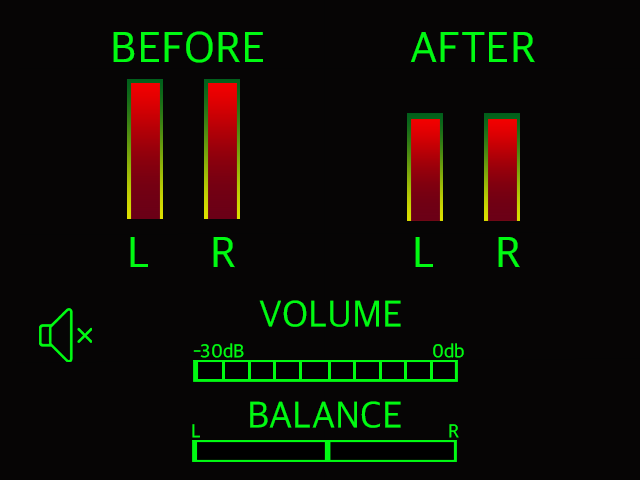
\includegraphics[scale=1]{UI.png}
       \caption{User interface}
        \label{fig:user interface}
\end{figure}




%% Remove the text above
